\chapter{UJI COBA DAN EVALUASI}
Pada bab ini akan dijelaskan tentang uji coba dan evaluasi dari implementasi sistem yang telah dilakukan pada bab 4.

\section{Lingkungan Uji Coba}
Lingkungan uji coba menggunakan sebuah komputer dengan spesifikasi perangkat keras dan perangkat lunak sebagai berikut.

\begin{enumerate}
	\item Perangkat Keras
	\begin{enumerate}
		\item Processor Intel® Core™ i5-3320M CPU @ 2.60GHz
		\item Random Access Memory 4GB
	\end{enumerate}
	\item Perangkat Lunak
	\begin{enumerate}
		\item Sistem Operasi Manjaro Illyria 18.0 64-bit
		\item Text Editor Visual Studio Code 1.29.1
		\item Bahasa Pemrograman C++
		\item g++ (GCC) 8.2.1 20181127
	\end{enumerate}
\end{enumerate}

\section{Uji Coba Kebenaran}
Subbab ini menjelaskan pengujian program untuk penyelesaian permasalahan \problem. Uji coba dilakukan untuk mendapatkan status \textit{Accepted} pada situs penilaian daring SPOJ dengan cara mengirim program ke \problem\cite{PT07G}.

\subsection{Uji Coba Kebenaran Lokal}
Uji coba lokal dilakukan dengan menjalankan program untuk menguji apakah program dapat berjalan tanpa \textit{error} dan menghasilkan \textit{graceful labelling} sesuai data masukan yang diberikan.

\subsubsection{Data Uji Coba Kebenaran Lokal}
Data yang digunakan untuk uji coba kebenaran lokal adalah data \textit{general tree} yang dibuat pada situs \textit{SPOJToolkit}\cite{SPOJTOOLKIT}. Terdapat 27 data yang masing-masing berisi data \textit{general tree} mulai dari satu \textit{node} hingga 27 \textit{node}.

\subsubsection{Skenario Uji Coba Kebenaran Lokal}
Uji coba dilakukan dengan menjalankan program dan melihat apakah program dapat berjalan tanpa \textit{error} dan dapat menghasilkan \textit{graceful labelling} dari data masukan.

\subsubsection{Evaluasi Kebenaran Uji Coba Lokal}
Evaluasi dilakukan dengan mengecek label yang didapat dari hasil program. Keluaran program akan dianggap benar apabila label yang dihasilkan program sesuai dengan ketentuan yang diberikan yaitu bersifat \textit{graceful} terhadap \textit{tree} masukan. Hasil uji coba dengan 27 masukan dapat dilihat pada Lampiran A.

Dari hasil pengujian diatas membuktikan bahwa program mampu menghasilkan \textit{graceful labelling} untuk \textit{tree} masukan. Contoh salah satu proses pencarian solusi untuk input dengan jumlah \textit{node} 12 dapat dilihat pada Gambar \ref{fig:uji_coba_1} - Gambar \ref{fig:uji_coba_11}.
\par Gambar \ref{fig:uji_coba_1} menunjukan kondisi awal \textit{program} yaitu nilai label awal berupa nilai \textit{node} dikurangi satu dan belum ada langkah pada riwayat langkah. Pada contoh ini jumlah nilai \textit{edge} awal yang unik bernilai 5.

\begin{figure}[ht]
	\centering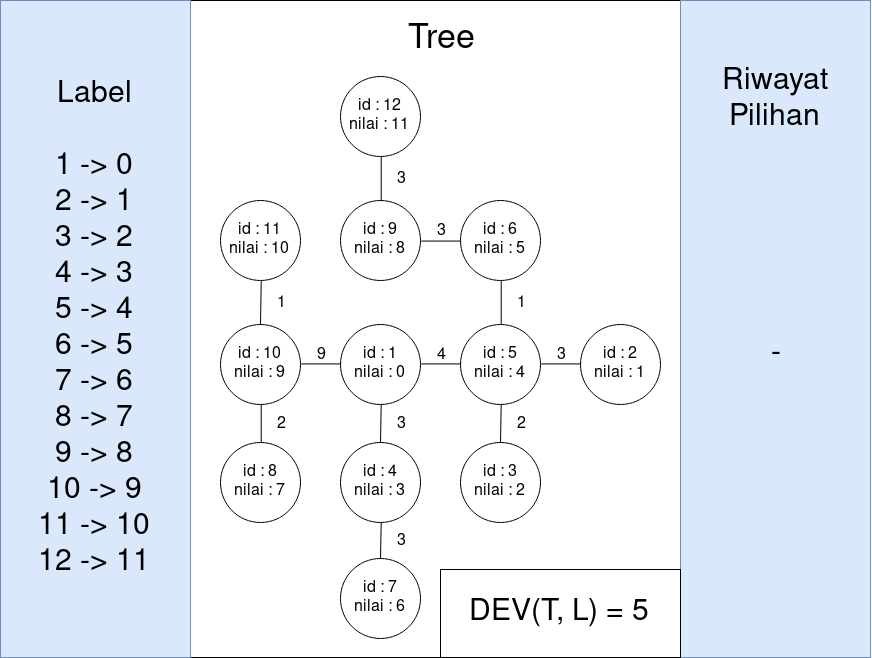
\includegraphics[width=1\textwidth]{bab5/figures/uji_coba_1.png}
	\caption{Kondisi awal program}
	\label{fig:uji_coba_1}
\end{figure}

Proses pencarian kondisi tetangga selanjutnya menemukan bahwa dengan melakukan proses $ SWAP(L, 1, 9) $ akan memiliki nilai yang lebih baik dari sebelumnya yaitu 6, maka program menukar nilai dari \textit{node} dengan id 1 dan \textit{node} dengan id 9. Program juga mencatat bahwa langkah penukaran antara \textit{node} dengan id 1 dan \textit{node} dengan id 9 telah dipilih saat ini. Kondisi setelah proses penukaran pertama dapat dilihat pada Gambar \ref{fig:uji_coba_2}.

\begin{figure}[ht]
	\centering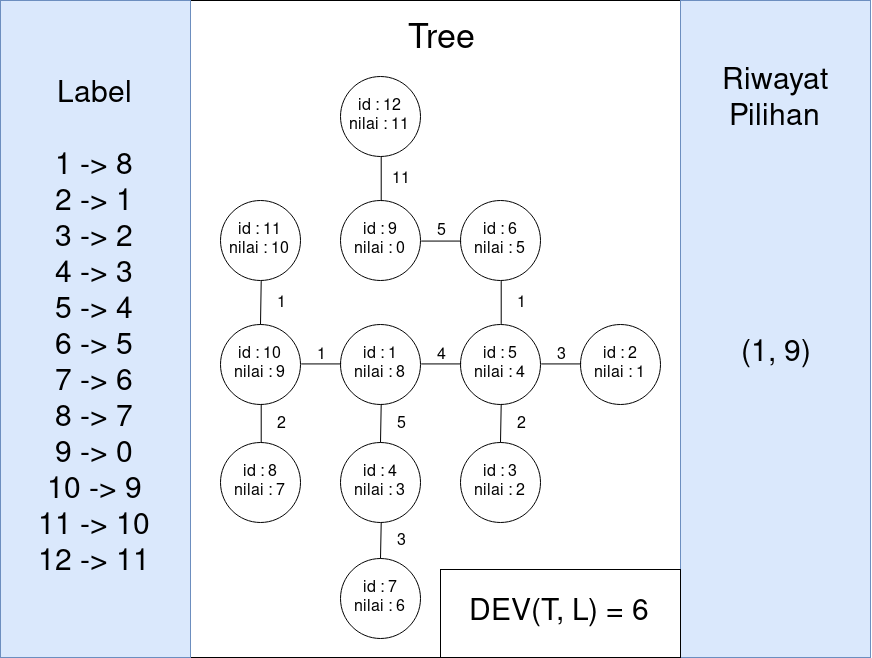
\includegraphics[width=1\textwidth]{bab5/figures/uji_coba_2.png}
	\caption{Kondisi setelah penukaran pertama}
	\label{fig:uji_coba_2}
\end{figure}

Proses pencarian kondisi tetangga selanjutnya menemukan bahwa dengan melakukan proses $ SWAP(L, 1, 11) $ akan memiliki nilai yang lebih baik dari sebelumnya yaitu 7, maka program menukar nilai dari \textit{node} dengan id 1 dan \textit{node} dengan id 11. Program juga mencatat bahwa langkah penukaran antara \textit{node} dengan id 1 dan \textit{node} dengan id 11 telah dipilih saat ini. Kondisi setelah proses penukaran kedua dapat dilihat pada Gambar \ref{fig:uji_coba_3}.

\begin{figure}[ht]
	\centering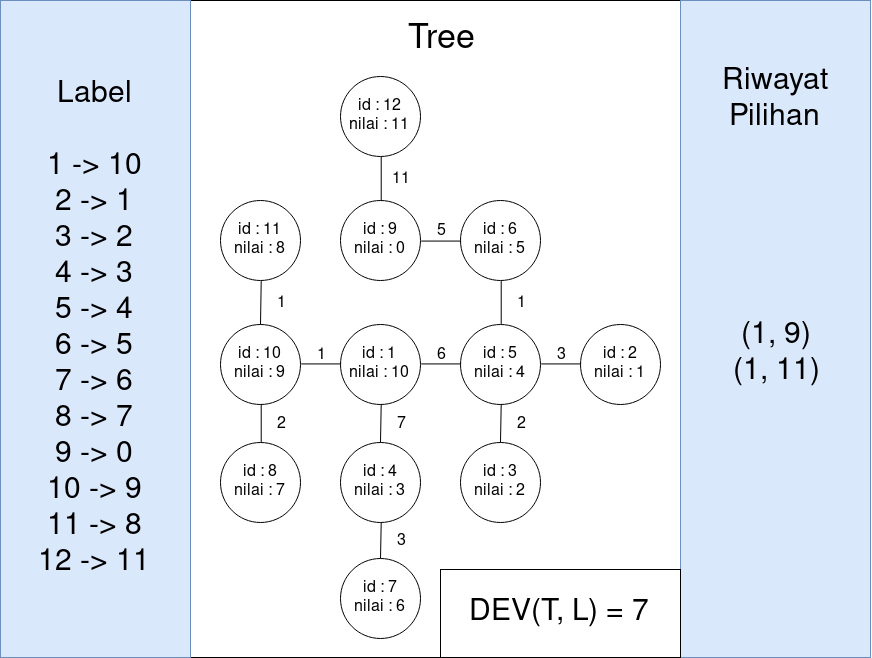
\includegraphics[width=1\textwidth]{bab5/figures/uji_coba_3.png}
	\caption{Kondisi setelah penukaran kedua}
	\label{fig:uji_coba_3}
\end{figure}

Proses pencarian kondisi tetangga selanjutnya menemukan bahwa dengan melakukan proses $ SWAP(L, 2, 5) $ akan memiliki nilai yang lebih baik dari sebelumnya yaitu 8, maka program menukar nilai dari \textit{node} dengan id 2 dan \textit{node} dengan id 5. Program juga mencatat bahwa langkah penukaran antara \textit{node} dengan id 2 dan \textit{node} dengan id 5 telah dipilih saat ini. Kondisi setelah proses penukaran ketiga dapat dilihat pada Gambar \ref{fig:uji_coba_4}.

\begin{figure}[ht]
	\centering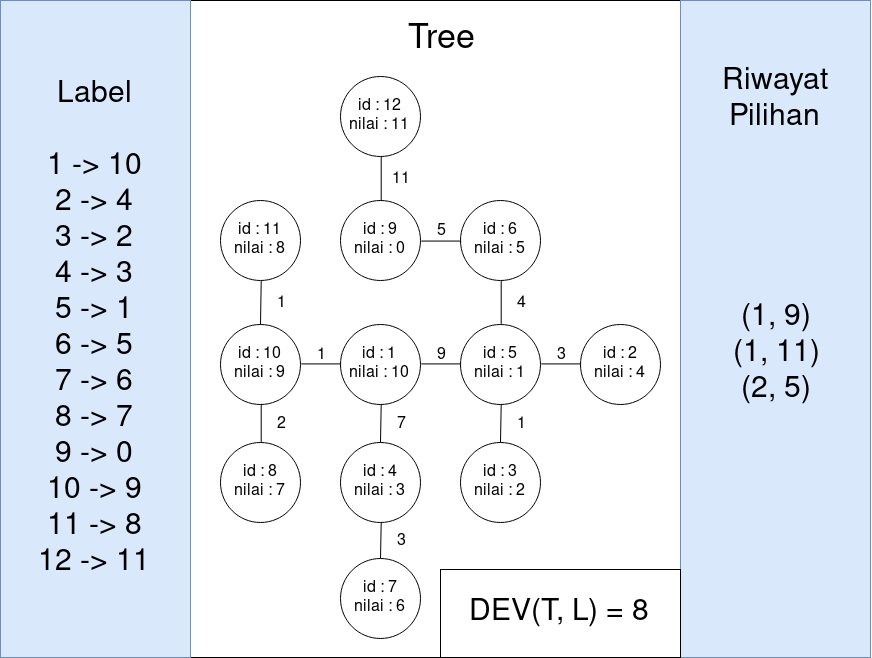
\includegraphics[width=1\textwidth]{bab5/figures/uji_coba_4.png}
	\caption{Kondisi setelah penukaran ketiga}
	\label{fig:uji_coba_4}
\end{figure}

Proses pencarian kondisi tetangga selanjutnya menemukan bahwa dengan melakukan proses $ SWAP(L, 2, 10) $ akan memiliki nilai yang lebih baik dari sebelumnya yaitu 9, maka program menukar nilai dari \textit{node} dengan id 2 dan \textit{node} dengan id 10. Program juga mencatat bahwa langkah penukaran antara \textit{node} dengan id 2 dan \textit{node} dengan id 10 telah dipilih saat ini. Kondisi setelah proses penukaran keempat dapat dilihat pada Gambar \ref{fig:uji_coba_5}.

\begin{figure}[ht]
	\centering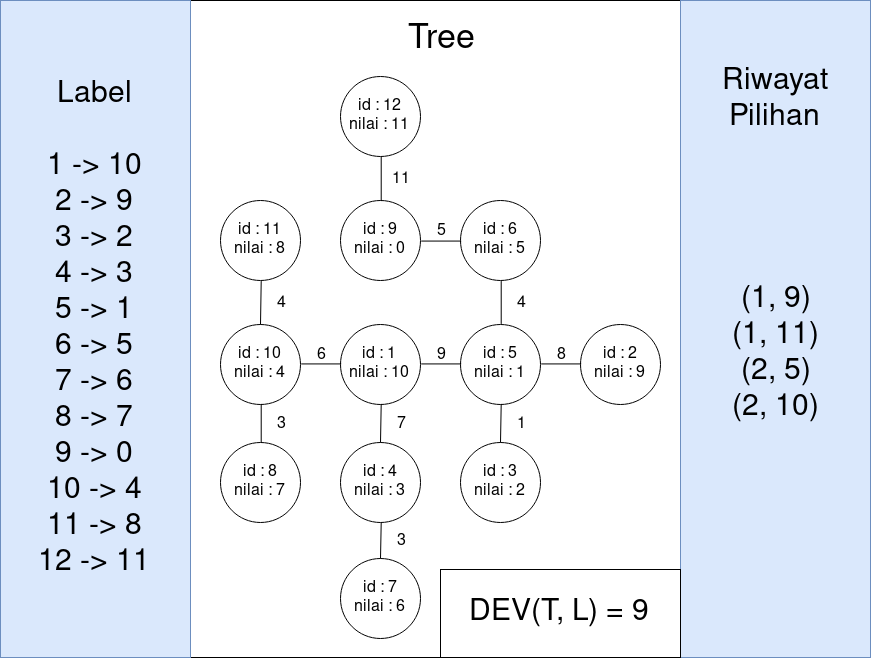
\includegraphics[width=1\textwidth]{bab5/figures/uji_coba_5.png}
	\caption{Kondisi setelah penukaran keempat}
	\label{fig:uji_coba_5}
\end{figure}

Proses pencarian kondisi tetangga selanjutnya menemukan bahwa dengan melakukan proses $ SWAP(L, 6, 7) $ akan memiliki nilai yang lebih baik dari sebelumnya yaitu 10, maka program menukar nilai dari \textit{node} dengan id 6 dan \textit{node} dengan id 7. Program juga mencatat bahwa langkah penukaran antara \textit{node} dengan id 6 dan \textit{node} dengan id 7 telah dipilih saat ini. Kondisi setelah proses penukaran kelima dapat dilihat pada Gambar \ref{fig:uji_coba_6}.

\begin{figure}[ht]
	\centering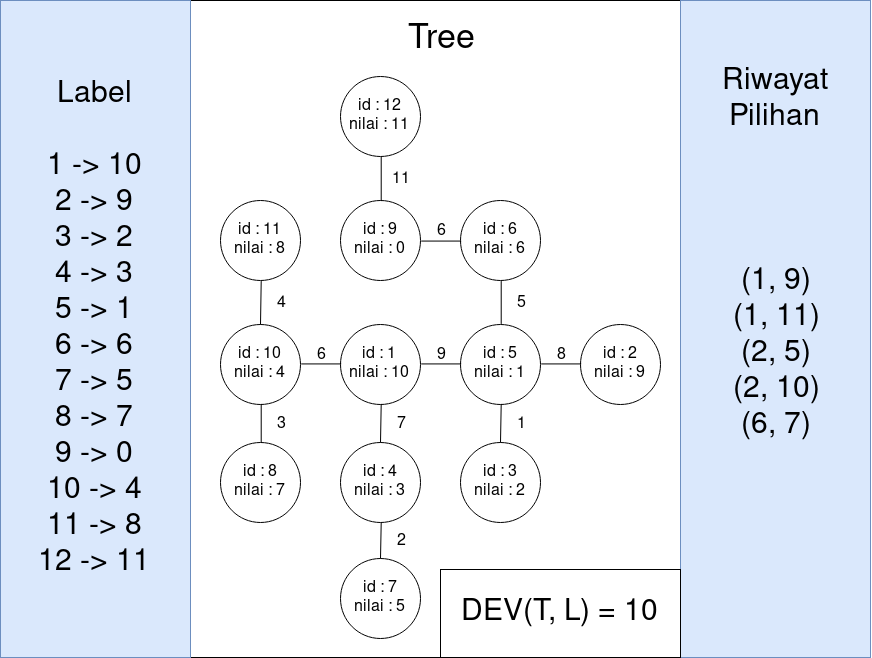
\includegraphics[width=1\textwidth]{bab5/figures/uji_coba_6.png}
	\caption{Kondisi setelah penukaran kelima}
	\label{fig:uji_coba_6}
\end{figure}

Proses pencarian kondisi tetangga selanjutnya tidak menemukan kondisi yang memiliki nilai lebih baik dari kondisi sekarang. Program memilih menukar nilai dari \textit{node} dengan id 2 dan \textit{node} dengan id 3 dikarenakan nilai kondisi hasil dari $ SWAP(L, 2, 3) $ menghasilkan nilai yang maksimal diantara semua kemungkinan tetangga kondisi sekarang yaitu 10 dan langkah $ (2,3) $ belum dipilih dalam 15 langkah sebelumnya. Program juga mencatat bahwa langkah penukaran antara \textit{node} dengan id 2 dan \textit{node} dengan id 3 telah dipilih saat ini. Kondisi setelah proses penukaran keenam dapat dilihat pada Gambar \ref{fig:uji_coba_7}.

\begin{figure}[ht]
	\centering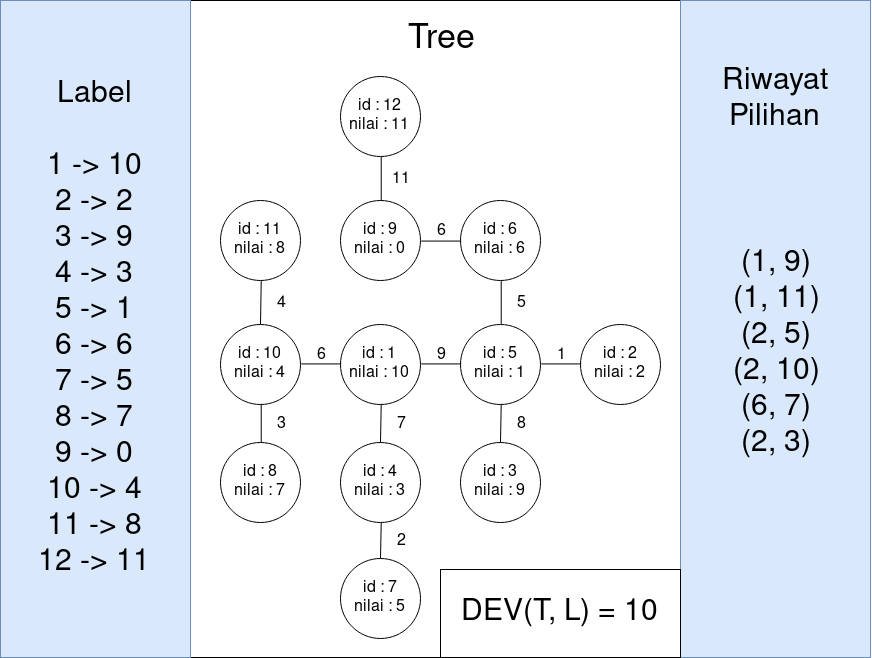
\includegraphics[width=1\textwidth]{bab5/figures/uji_coba_7.png}
	\caption{Kondisi setelah penukaran keenam}
	\label{fig:uji_coba_7}
\end{figure}

Proses pencarian kondisi tetangga selanjutnya tidak menemukan kondisi yang memiliki nilai lebih baik dari kondisi sekarang. Program memilih menukar nilai dari \textit{node} dengan id 2 dan \textit{node} dengan id 6 dikarenakan nilai kondisi hasil dari $ SWAP(L, 2, 6) $ menghasilkan nilai yang maksimal diantara semua kemungkinan tetangga kondisi sekarang yaitu 10 dan langkah $ (2,6) $ belum dipilih dalam 15 langkah sebelumnya. Program juga mencatat bahwa langkah penukaran antara \textit{node} dengan id 2 dan \textit{node} dengan id 6 telah dipilih saat ini. Kondisi setelah proses penukaran ketujuh dapat dilihat pada Gambar \ref{fig:uji_coba_8}.

\begin{figure}[ht]
	\centering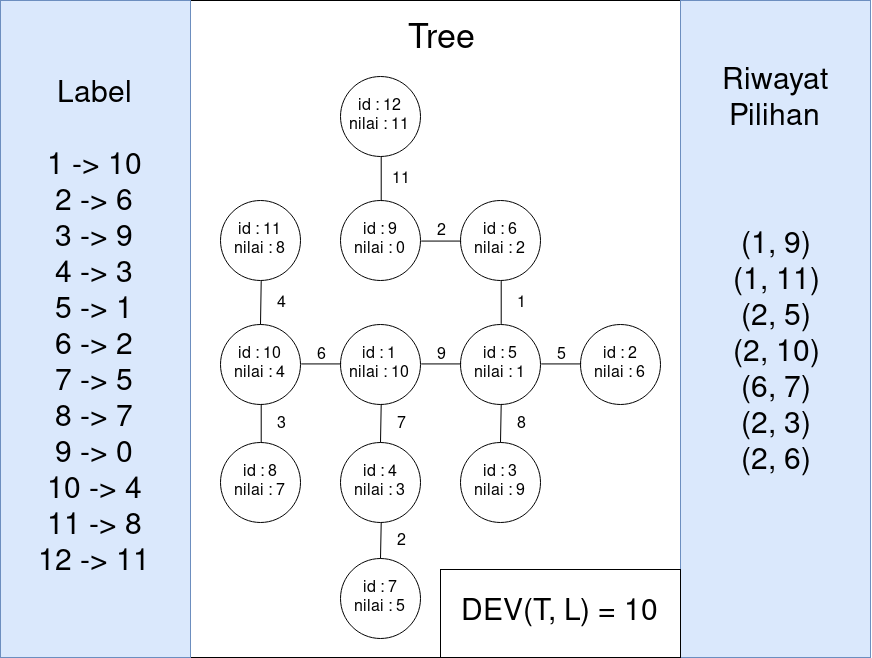
\includegraphics[width=1\textwidth]{bab5/figures/uji_coba_8.png}
	\caption{Kondisi setelah penukaran ketujuh}
	\label{fig:uji_coba_8}
\end{figure}

Proses pencarian kondisi tetangga selanjutnya tidak menemukan kondisi yang memiliki nilai lebih baik dari kondisi sekarang. Program memilih menukar nilai dari \textit{node} dengan id 3 dan \textit{node} dengan id 6 dikarenakan nilai kondisi hasil dari $ SWAP(L, 3, 6) $ menghasilkan nilai yang maksimal diantara semua kemungkinan tetangga kondisi sekarang yaitu 10 dan langkah $ (3,6) $ belum dipilih dalam 15 langkah sebelumnya. Program juga mencatat bahwa langkah penukaran antara \textit{node} dengan id 3 dan \textit{node} dengan id 6 telah dipilih saat ini. Kondisi setelah proses penukaran kedelapan dapat dilihat pada Gambar \ref{fig:uji_coba_9}.

\begin{figure}[ht]
	\centering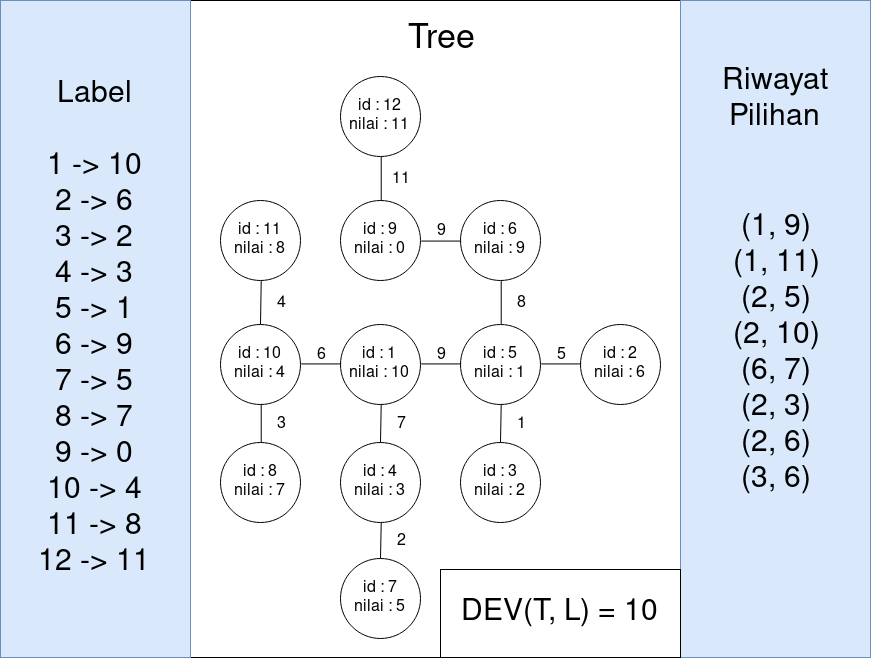
\includegraphics[width=1\textwidth]{bab5/figures/uji_coba_9.png}
	\caption{Kondisi setelah penukaran kedelapan}
	\label{fig:uji_coba_9}
\end{figure}

Proses pencarian kondisi tetangga selanjutnya tidak menemukan kondisi yang memiliki nilai lebih baik dari kondisi sekarang. Program memilih menukar nilai dari \textit{node} dengan id 1 dan \textit{node} dengan id 6 dikarenakan nilai kondisi hasil dari $ SWAP(L, 1, 6) $ menghasilkan nilai yang maksimal diantara semua kemungkinan tetangga kondisi sekarang yaitu 10 dan langkah $ (1,6) $ belum dipilih dalam 15 langkah sebelumnya. Program juga mencatat bahwa langkah penukaran antara \textit{node} dengan id 1 dan \textit{node} dengan id 6 telah dipilih saat ini. Kondisi setelah proses penukaran kesembilan dapat dilihat pada Gambar \ref{fig:uji_coba_10}.

\begin{figure}[ht]
	\centering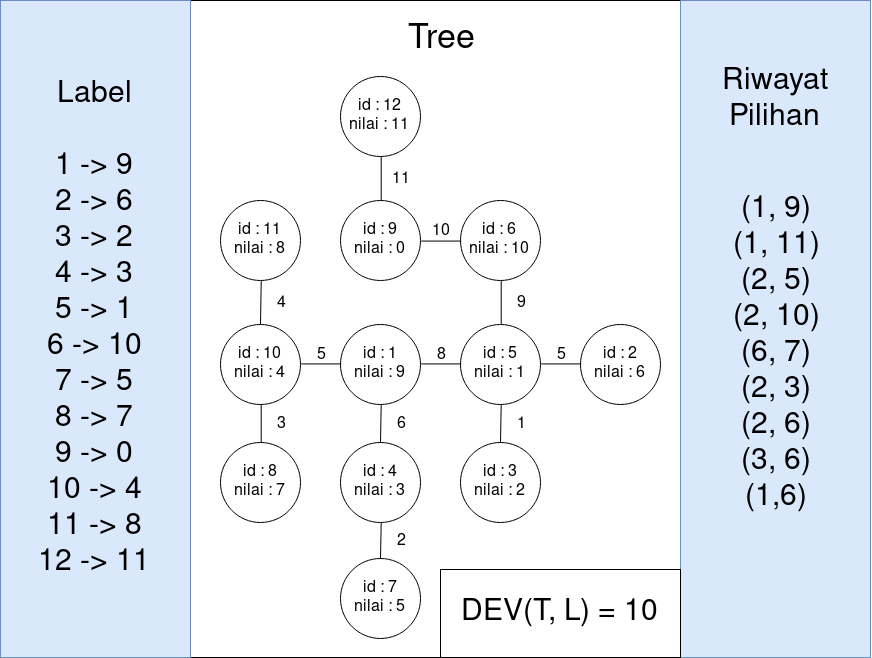
\includegraphics[width=1\textwidth]{bab5/figures/uji_coba_10.png}
	\caption{Kondisi setelah penukaran kesembilan}
	\label{fig:uji_coba_10}
\end{figure}

Proses pencarian kondisi tetangga selanjutnya tidak menemukan kondisi yang memiliki nilai lebih baik dari kondisi sekarang. Program memilih menukar nilai dari \textit{node} dengan id 2 dan \textit{node} dengan id 11 dikarenakan nilai kondisi hasil dari $ SWAP(L, 2, 11) $ menghasilkan nilai yang maksimal diantara semua kemungkinan tetangga kondisi sekarang yaitu 10 dan langkah $ (2,11) $ belum dipilih dalam 15 langkah sebelumnya. Program juga mencatat bahwa langkah penukaran antara \textit{node} dengan id 2 dan \textit{node} dengan id 11 telah dipilih saat ini. Kondisi setelah proses penukaran kesepuluh dapat dilihat pada Gambar \ref{fig:uji_coba_11}.

\begin{figure}[ht]
	\centering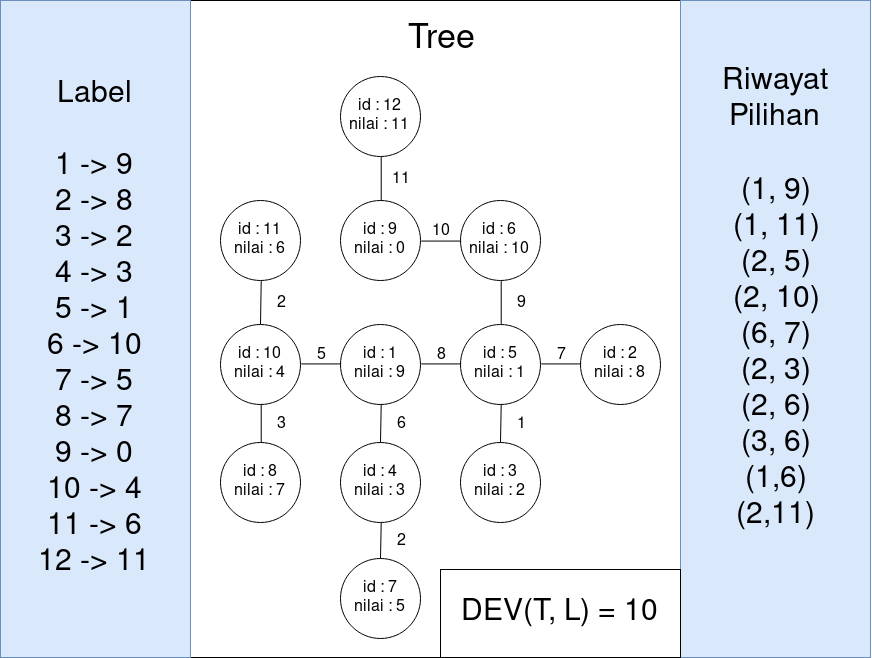
\includegraphics[width=1\textwidth]{bab5/figures/uji_coba_11.png}
	\caption{Kondisi setelah penukaran kesepuluh}
	\label{fig:uji_coba_11}
\end{figure}

Proses pencarian kondisi tetangga selanjutnya menemukan bahwa dengan melakukan proses $ SWAP(L, 3, 7) $ akan memiliki nilai yang lebih baik dari sebelumnya yaitu 11, maka program menukar nilai dari \textit{node} dengan id 3 dan \textit{node} dengan id 7. Program juga mencatat bahwa langkah penukaran antara \textit{node} dengan id 3 dan \textit{node} dengan id 7 telah dipilih saat ini. Kondisi setelah proses penukaran kesebelas dapat dilihat pada Gambar \ref{fig:uji_coba_12}.

\begin{figure}[ht]
	\centering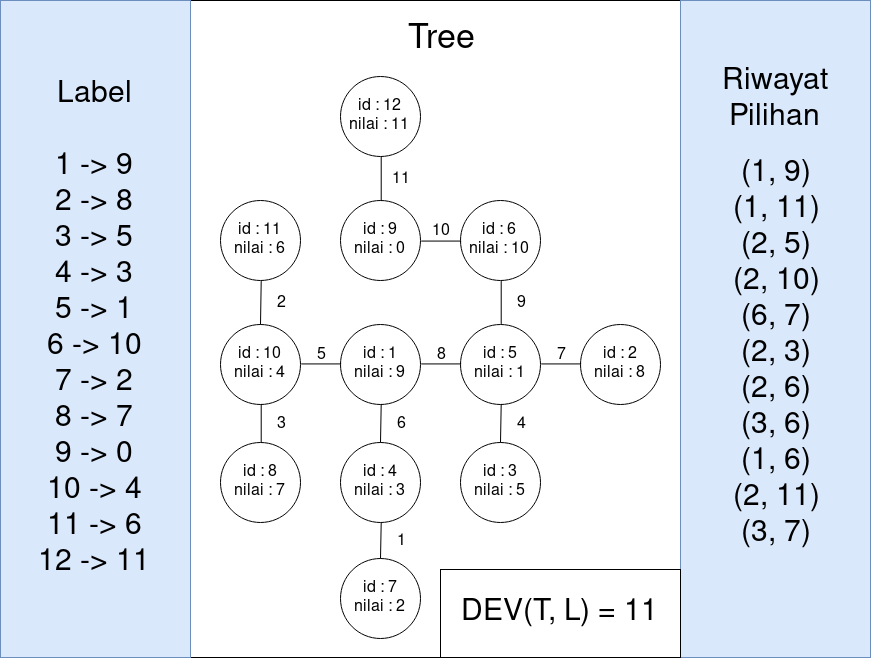
\includegraphics[width=1\textwidth]{bab5/figures/uji_coba_12.png}
	\caption{Kondisi setelah penukaran kesebelas}
	\label{fig:uji_coba_12}
\end{figure}

Setelah proses penukaran kesebelas kondisi sekarang telah memiliki 11 nilai \textit{edge} yang unik maka kondisi label sekarang telah memenuhi ketentuan \textit{graceful labelling} yang diinginkan. Hal ini menunjukan program berhasil menyelesaikan permasalahan khususnya pada masukan dengan \textit{tree} dengan \textit{node} berjumlah 12.

\subsection{Uji Coba Kebenaran Situs Penilaian Daring SPOJ}
Uji coba pada situs penilaian daring SPOJ dilakukan dengan mengirim kode sumber ke situs \problem\cite{PT07G}.

\subsubsection{Data Uji Coba Kebenaran Situs Penilaian Daring SPOJ}
Data yang digunakan pada uji coba ini adalah data yang ada pada situs \problem\cite{PT07G} sehingga data masukan yang digunakan untuk pengujian tidak dapat diketahui.

\subsubsection{Evaluasi Uji Coba Kebenaran Situs Penilaian Daring SPOJ}
Evaluasi dilakukan dengan melihat status pengumpulan yang didapatkan pada \problem\cite{PT07G}. Hasil uji kebenaran situs penilaian daring SPOJ dapat dilihat pada Gambar \ref{fig:status_spoj}

\begin{figure}[ht]
	\centering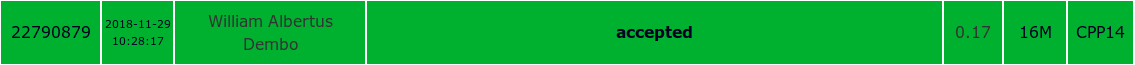
\includegraphics[width=1\textwidth]{bab5/figures/status_spoj.png}
	\caption{Hasil uji coba kebenaran situs penilaian daring SPOJ}
	\label{fig:status_spoj}
\end{figure}

\section{Uji Coba Kinerja}
Subbab ini menjelaskan pengujian kinerja program pada Tugas Akhir ini untuk menyelesaikan permasalahan \textit{graceful labelling} pada \textit{general tree}. Uji coba kinerja dilakukan untuk mengetahui gambaran kinerja program pada tugas akhir ini dan mendapatkan peringkat terbaik pada situs penilaian daring SPOJ.

\subsection{Uji Coba Kinerja Lokal}
Uji coba kinerja lokal dilakukan dengan menjalankan program pada tugas akhir ini dan program yang menggunakan algoritma naif untuk mendapatkan perbandingan kinerja diantara kedua program.

\subsubsection{Data Uji Coba Kinerja Lokal}
Data yang digunakan untuk uji coba kinerja adalah data \textit{general tree} yang dibuat pada situs \problem\cite{SPOJTOOLKIT}. Terdapat 100 data masing-masing 10 data untuk \textit{general tree} dengan jumlah \textit{node} satu hingga 10.

\subsubsection{Skenario Uji Coba Kinerja Lokal}
Uji coba dilakukan dengan menjalankan program pada Tugas Akhir ini dan program dengan algoritma naif kemudian dilakukan pencatatan waktu yang dibutuhkan program untuk menyelesaikan permasalahan.

\subsubsection{Evaluasi Uji Coba Kinerja Lokal}
Evaluasi dilakukan dengan membandingkan waktu yang dibutuhkan masing-masing program untuk menyelesaikan permasalahan. Waktu yang ditampilkan merupakan rata-rata waktu yang dibutuhkan untuk \textit{general tree} dengan masing-masing jumlah \textit{node} dari satu hingga 10. Data hasil uji coba kinerja dapat dilihat pada Tabel \ref{table:uji_coba_kinerja} dan grafik hasil uji coba kinerja dapat dilihat pada Gambar \ref{fig:grafik_uji_coba_kinerja}.

\begin{table}[ht!]
	\centering
	\begin{tabularx}{0.6\textwidth}{|l|l|X|}
	\hline
								 & \multicolumn{2}{l|}{Waktu (mikrodetik)} \\ \cline{2-3} 
	Jumlah Node					 & Naive          & Tugas Akhir       \\ \hline
	1                            & 9       		  & 7                 \\ \hline
	2                            & 14       	  & 6       	      \\ \hline
	3                            & 9       		  & 11          	  \\ \hline
	4                            & 19       	  & 18     		      \\ \hline
	5                            & 50       	  & 27          	  \\ \hline
	6                            & 354       	  & 37     	          \\ \hline
	7                            & 1193       	  & 88        	      \\ \hline
	8                            & 8026           & 104          	  \\ \hline
	9                            & 42386          & 514          	  \\ \hline
	10                           & 434387         & 574          	  \\ \hline
	11                           & -     	      & 1769          	  \\ \hline
	12                           & -        	  & 1850          	  \\ \hline
	13                           & -        	  & 3764          	  \\ \hline
	14                           & -       		  & 3311          	  \\ \hline
	15                           & -       		  & 5459          	  \\ \hline
	16                           & -              & 7568          	  \\ \hline
	17                           & -         	  & 10495          	  \\ \hline
	18                           & -     	      & 11045          	  \\ \hline
	19                           & -         	  & 15168          	  \\ \hline
	20                           & -         	  & 24742          	  \\ \hline
	21                           & -	          & 40080          	  \\ \hline
	22                           & -    	      & 62929          	  \\ \hline
	23                           & -        	  & 100159            \\ \hline
	24                           & -  	          & 99732          	  \\ \hline
	25                           & -     	      & 121648            \\ \hline
	26                           & -         	  & 152602            \\ \hline
	27                           & -              & 212134            \\ \hline
	\end{tabularx}
	\caption{Tabel data hasil uji coba kinerja lokal}
	\label{table:uji_coba_kinerja}
\end{table}

\begin{figure}[ht!]
	\centering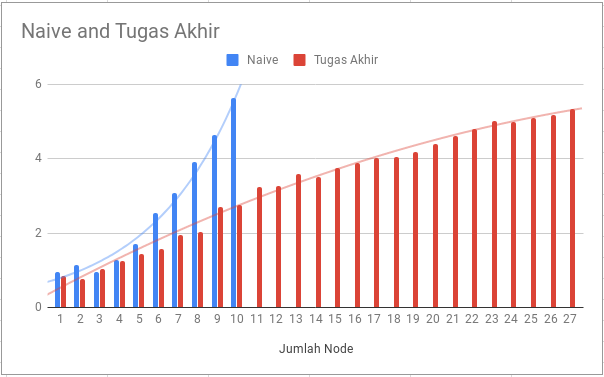
\includegraphics[width=\textwidth]{bab5/figures/grafik_uji_coba_kinerja_log_new.png}
	\caption{Grafik uji coba kinerja lokal dalam logaritmik}
	\label{fig:grafik_uji_coba_kinerja}
\end{figure}

\subsection{Uji Coba Kinerja Situs Penilaian Daring SPOJ}
Uji coba kinerja pada situs penilaian daring SPOJ dilakukan dengan mengirim program ke situs SPOJ \problem\cite{PT07G}. Beberapa program yang dikirimkan pada situs penilaian daring SPOJ merupakan program yang masing-masing variabel bebasnya memiliki nilai yang berbeda.

\subsubsection{Data Uji Coba Kinerja Situs Penilaian Daring SPOJ}
Data yang digunakan pada uji coba ini adalah data yang ada pada situs \problem\cite{PT07G} sehingga data masukan yang digunakan untuk pengujian tidak dapat diketahui.

\subsubsection{Skenario Uji Coba Kinerja Situs Penilaian Daring SPOJ}
Uji coba dilakukan dengan mengubah-ubah nilai dari komponen nilai batasan tabu atau nilai $ M $ pada Bab \ref{algoritma_solusi} dan mengirim program ke situs \problem\cite{PT07G}.

\subsubsection{Evaluasi Uji Coba Kinerja Situs Penilaian Daring SPOJ}
Evaluasi dilakukan dengan melihat waktu yang dibutuhkan program pada situs \problem\cite{PT07G}. Hasil uji kinerja pada program menggunakan variabel bebas $ M $ pada situs penilaian daring SPOJ dapat dilihat pada Tabel \ref{table:uji_coba_kinerja_spoj}. Pringkat kinerja waktu pada situs penilaian daring dapat dilihat pada Gambar \ref{fig:spoj_rank}.

\begin{table}[ht!]
	\centering
	\begin{tabularx}{0.6\textwidth}{|l|X|}
	\hline
	Nilai M						& Waktu Kinerja (detik) \\ \hline
	5							& TLE (>1) \\ \hline
	10							& TLE (>1) \\ \hline
	15							& 0.17 \\ \hline
	20							& 0.22 \\ \hline
	25							& 0.24 \\ \hline
	30							& 0.26 \\ \hline
	\end{tabularx}
	\caption{Tabel data hasil uji coba kinerja situs penilaian daring SPOJ}
	\label{table:uji_coba_kinerja_spoj}
\end{table}

\begin{figure}[ht!]
	\centering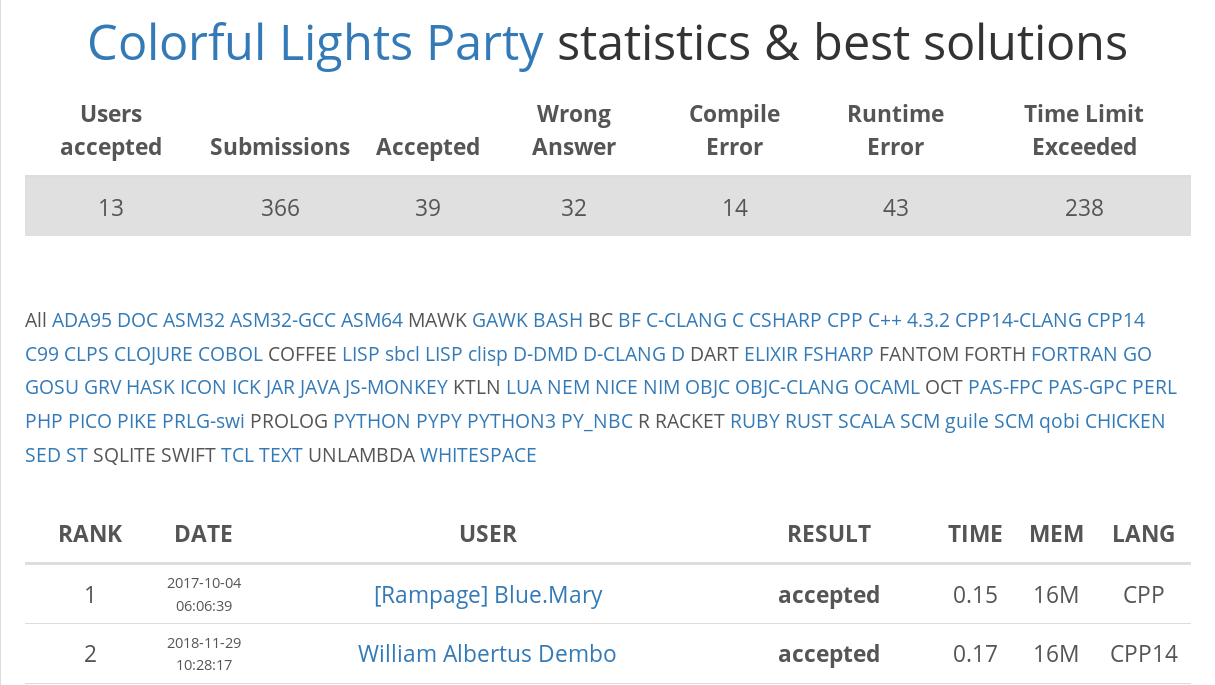
\includegraphics[width=\textwidth]{bab5/figures/spoj_rank.png}
	\caption{Peringkat kinerja pada situs penilaian daring SPOJ}
	\label{fig:spoj_rank}
\end{figure}